%!TEX root = ../thesis.tex
%*******************************************************************************
%*********************************** First Chapter *****************************
%*******************************************************************************

\chapter{Discussion}  %Title of the First Chapter

\ifpdf
    \graphicspath{{Chapter7/Figs/Raster/}{Chapter7/Figs/PDF/}{Chapter7/Figs/}}
\else
    \graphicspath{{Chapter7/Figs/Vector/}{Chapter7/Figs/}}
\fi


%********************************** %First Section  **************************************
\section{Converting iPG into Blood Flow} %Section - 7.1 
\label{section discussion 1}
As it has been discussed in this document, there are two ways to calculate blood flow from the iPG data. Initially, it is needed to model the segment of the body as a cylinder. Luckily, most of the body parts can be expressed as this geometrical figure. For this study, a device was designed to measure the change of volume in the forearm. Eventually, this could be calibrated to work in other parts of the body such as lower extremities. 

The study performed in this document seeks to demonstrate how the iPG data could help to detect changes in venous and arterial circulation. According to the literature, iPG is a method used to quantify blood flow from the principle that the impedance of a body part is directly proportional to its volume as described by Nyober's equation  (see equation \ref{eq:Nyober}).  Hence, since the 1970's this theory has been tested assuring the effectivity of the method. 

There are different contributors to the impedimetric signal. One of them are the tissues such as fat, muscle, blood or even bone. Most of this organs are static, meaning that if the movement is limited the only reading will be equivalent to the impedance reading of these organs. This resistive value is known as basal impedance.  However,  the circulatory system is dynamic and create small changes during the cardiac cycle.  When the ventricles contract this produces a small increment of the size of the vessels by filling them with blood. 
\mynote{check a reference about circulatory and added to this section. Also, check how to related to the medical background}. Therefore, this increment in blood within the tissue creates an raise of volume, and change of volume in time can be converted into the flow rate.

The first method to measure blood flow is called venous occlusion plethysmography \cite{wilkinson2001venous}. This approach inquires the increment of impedance when an occlusion is performed in the upper part of a limb using a cuff. The most common occlusion level is about \SI{40}{\mmHg} for a determined time. This occlusion could be for some seconds until minutes depending on the study to be done. 

By occluding the venous return and not altering the arterial flow, blood can enter into the limb but cannot leave.  As a result, there is a linear increase in the volume of the limb. Hence, this gain of capacity can be quantified by the impedimetric method which is clearly perceptible in the variation of the DC component of the signal. In fact, this is because the blood begins to cluster in the limb. As the blood's population increases, the conductivity of the forearm's section also rises in volume. Therefore, the resistivity proportionally decreases. 

During the experiment presented in this document the venous occlusion occurred throughout region 1 and region 2.  As shown by figure \ref{fig:rb:all_participants}, it is clear that most of the participants experience a variation in the basal impedance readings.  However, some of them were affected by motion which produced changes in the trend, like in participant 1. However, in most of the participants was seen this linear decrease of impedance. 

In a similar situation, there was a reduction in the forearm's inflow when the brachial artery in the upper arm was partially occluded. Performing this action stops the venous total return but also alters the incoming arterial flow \mynote{Check a paper about changing the elasticity of a tube changes its flow}. This effect was verified when reviewing the Doppler ultrasound data. In figure xxx 5.16 can be seen that the participants experienced a decrease in their flow. As a result, again the forearms volume increased shifting the forearm's impedance. It was noticed that when this occurs, the basal impedance decreases in a larger slope. This greater slope might be an indication of a higher laminar flow coming from the artery \mynote{Check what happens during arterial occlusion}.  

All along total occlusion seemed that there was not clear change in the basal impedance.  Because both arterial and venous flow have been blocked, there was not blood flow of any kind in the arm section. All the instruments replicated this event. However, only the Doppler ultrasound was able to reproduce a biological zero, the rest of the instruments showed some level of noisy data.   Therefore, this is the real value of the basal impedance where all the tissues with their blood content were measured.  

%********************************** %Second Section  *************************************
\section{How much is related the iPG blood flow with other instruments?} %Section - 7.2
\label{section discussion 4}

%********************************** % Third Section  *************************************
\section{Option to evaluate blood flow using iPG DC and AC waveforms}  %Section - 7.3 
\label{section discussion 3}


\begin{figure}[!htpb]
	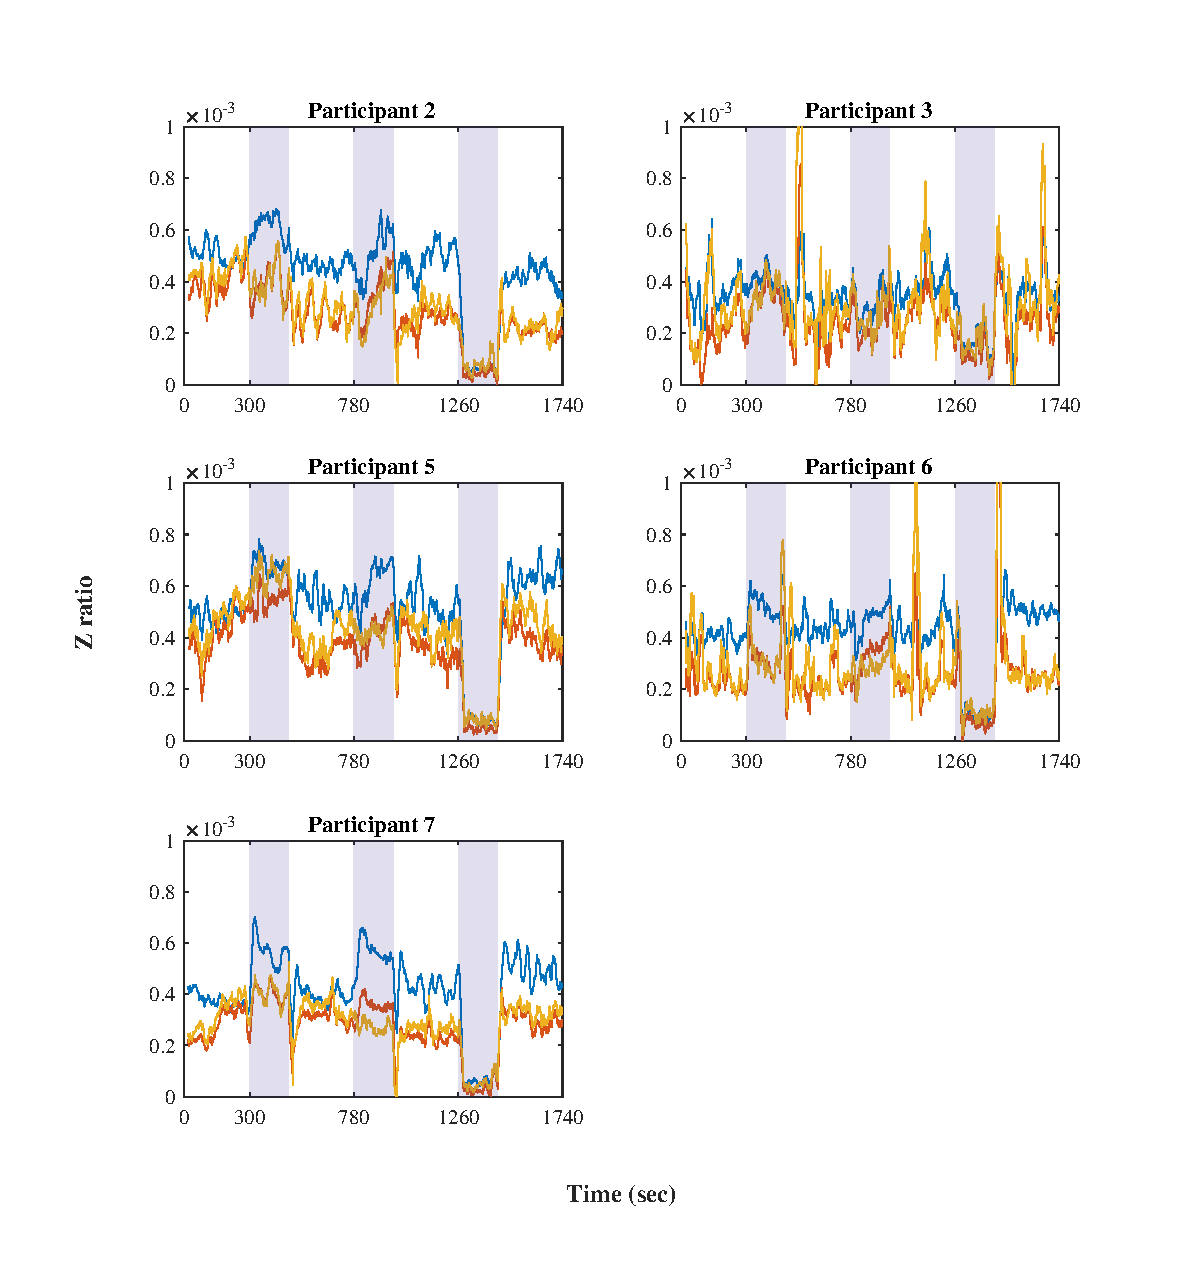
\includegraphics[width=1\textwidth,keepaspectratio]{figure1}    
	\caption[Bland and Altman plot of the relation between LDF and iPG]{Bland and Altman~\cite{bland1986statistical} plot of the relation between LDF and iPG. Data set corresponds to participants 2, 5, 6 and 7. The data has been normalised comparing the amplitude of both measurements. The different regions has been plotted with various colours and symbols to differentiate every event. The dotted line represents the perfect agreement, the dark line is the linear regression.}
	\label{fig:ratio Z}
\end{figure}

\begin{figure}[!htpb]
	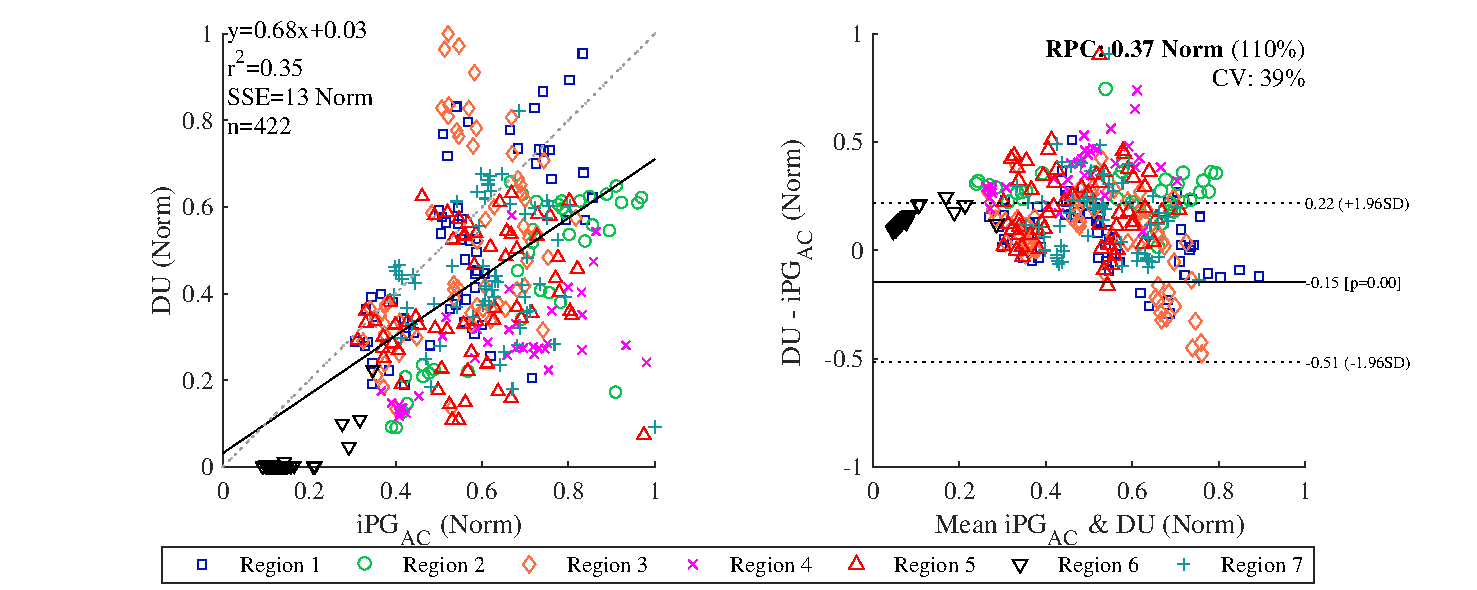
\includegraphics[width=1\textwidth,keepaspectratio]{figure2}    
	\caption[Bland and Altman plot of the relation between LDF and iPG]{Bland and Altman~\cite{bland1986statistical} plot of the relation between LDF and iPG. Data set corresponds to participants 2, 5, 6 and 7. The data has been normalised comparing the amplitude of both measurements. The different regions has been plotted with various colours and symbols to differentiate every event. The dotted line represents the perfect agreement, the dark line is the linear regression.}
	\label{fig:ration Z bar}
\end{figure}
